\chapter{Raster image correlation spectroscopy}
\label{ch:rics}

\lettrine[lines=2, lhang=0.33, loversize=0.25]{R}{aster image
correlation spectroscopy} is based on merging the concepts of \ac{LSCM},
\ac{FCS} and \ac{ICS}\citep{Brown_08_JMicrosc_229_p78,Digman_05_BiophysJ_89_p1317}. 
Detailed reviews are available covering the method and how it
relates to other \ac{FCS}-based methods
\citep{Digman_11_AnnuRevPhysChem_62_p645,Haustein_07_AnnuRevBiophysBiomolStruct_36_p151}.
Here, a brief overview of the concepts behind \ac{RICS} and to
our modification to this method are presented.
\section{Fundamentals}
\subsection{Image acquisition}
Fundamental to the method of \acs{RICS} is the realization that in an image
obtained by a \ac{LSCM}, pixels on the image
are not only separated in space but also in time \citep{Digman_05_BiophysJ_89_p1317}. Photons emitted by
excited fluorescent molecules are recorded as raster images as the
mirrors scan the laser beam on the specimen.  
When recording a two dimensional raster image, the laser beam moves 
along one image axis ($\xi$), spending $\tau_d$ seconds acquiring each pixel on
the line (dwell time), then flies back to the beginning of the line with
flyback time $\tau_f$, moves one pixel forward in the other axis($\psi$) and records
the second line. This sequential processes is repeated until the whole
image has been scanned line by line (\F{~\ref{fig:rics_theory1}}),
resulting in a rectangular grid of pixels separated in space and time.

\begin{figure}%[h!]
  \centering
    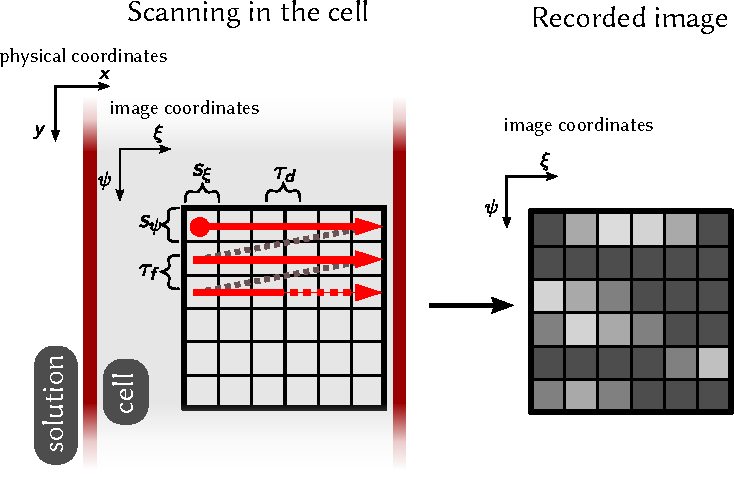
\includegraphics[width=10cm]{figures/rics_theory_1.pdf}
    \caption[\acs{RICS} image acquisition]{
    \acs{RICS} image acquisition. A raster image
    consisting of a grid of pixels is acquired within a cell. Pixels are
    separated by $s_\xi$,$s_\psi$ $\mu$m spatially and by $\tau_d$,$n_\xi\times
    \tau_d + \tau_f$ $\mu$s temporally in the $\xi$ and $\psi$
    directions,
    respectively. In the default case the image coordinates $\xi$, $\psi$
    align with the physical coordinates $x$, $y$. The image obtained (on
    the right)
    shows traces of diffusing molecules within the cell.}
  \label{fig:rics_theory1}
%The autocorrelation at shift vector $\Delta \mathbf{h}=(\xi,\psi)$ for an image with
%fluorescence values $F(\mathbf{p})$ at location $\mathbf{p} = (x,y)$ is given by:
%{\small
\end{figure}
\subsection{Correlation function \& diffusion}
By calculating the \ac{CF} of the scanned image
it is possible to extract information about the space-time relationship
between the pixels and to characterize, for example, reaction kinetics, translational and 
rotational diffusion, conformational dynamics, molecular flow, etc.
\citep{Digman_11_AnnuRevPhysChem_62_p645,Lakowicz_06_Springer,Haustein_07_AnnuRevBiophysBiomolStruct_36_p151}.
This can be done by fitting experimentally obtained \ac{CF} s with
theoretical \ac{CF} curves derived for the phenomenon being observed.
In this paper we focus on applying \acs{RICS} on analysis of diffusion of
fluorescent dyes.
\begin{figure}%[t]
  \centering
    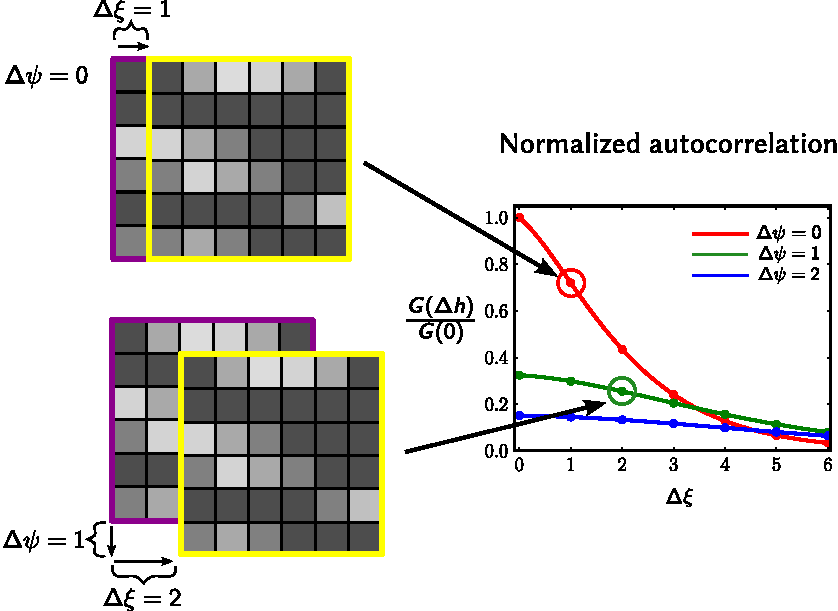
\includegraphics[width=10cm]{figures/rics_theory_2.pdf}
    \caption[Correlation function calculation]{
    The \acl{CF} $G(\Delta \mathbf{h})$ for the shift
    $\Delta \mathbf{h}=(\Delta\xi,\Delta\psi)$ is calculated by
    shifting a copy of the original image, multiplying the fluorescence
    values and averaging over the image. Arrows indicate the
    location of the correlation value for the shifts shown. The
    \ac{CF} here is normalized to the zero-shift
    correlation $G(0)$ from \Eq{~\ref{eq:G_0}}.}
  \label{fig:rics_theory2}
%The autocorrelation at shift vector $\Delta \mathbf{h}=(\xi,\psi)$ for an image with
%fluorescence values $F(\mathbf{p})$ at location $\mathbf{p} = (x,y)$ is given by:
%{\small
\end{figure}

The correlation function
$G(\Delta\xi,\Delta\psi,\Delta\zeta)$ indicates the
similarity of an image to a copy of itself shifted by $\Delta\xi$ in the
$\xi$
direction, $\Delta\psi$ in the $\psi$ direction (see
\F{~\ref{fig:rics_theory2}}) and, in case a 3D stack
of images is analyzed, $\Delta\zeta$ in the
$\zeta$ direction (otherwise $\Delta\zeta=0$).  

The \ac{CF} for a given shift is calculated by
multiplying the fluorescence values in the original image with
values in the shifted image and averaging over all the pixels. The
result is normalized to average image fluorescence squared:

\begin{align}  
  \label{eq:first}
  &G(\Delta\xi,\Delta\psi,\Delta\zeta)= \\
  &\quad \frac{\langle F(\xi,\psi,\zeta)
  \cdot F(\xi + \Delta\xi, \psi +
  \Delta\psi,\zeta+\Delta\zeta)\rangle_{\xi,\psi,\zeta}}{\langle F
  \rangle_{\xi,\psi,\zeta}^2} - 1,\nonumber
\end{align}
where $\langle\ldots\rangle$ signifies averaging over the whole
image.

The \ac{CF} can also be calculated in terms of
fluorescence fluctuations from the average $\delta F=F-\langle F
\rangle$ by substituting $F=\delta F +\langle F \rangle$ into
\Eq{~\ref{eq:first}}:
\begin{align*}
  &G(\Delta\xi,\Delta\psi,\Delta\zeta)= \\
  &\qquad\frac{\langle \delta F(\xi,\psi,\zeta) \cdot \delta F(\xi +\Delta
  \xi, \psi +
  \Delta\psi,\zeta+\Delta\zeta)\rangle_{\xi,\psi,\zeta}}{\langle F
  \rangle_{\xi,\psi,\zeta}^2}.
\end{align*}
%}

It is more convenient to present the \ac{CF} in vector form with image shift vector
$\Delta \mathbf{h}=\left[\Delta\xi,\Delta\psi,\Delta\zeta\right]$ and
position vector $\mathbf{h} = [\xi,\psi,\zeta]$:
\begin{equation}\label{eq:G_def}
 G(\Delta \mathbf{h}) = \frac{\langle \delta F(\mathbf{h}) \cdot
 \delta F(\mathbf{h} +\Delta \mathbf{h})\rangle_{\mathbf{h}}}{\langle
 F \rangle_{\mathbf{h}}^2}.
\end{equation}


The physical coordinates corresponding to image coordinates $\mathbf{h}$
are $\mathbf{p} =
\mathbf{p_0}+\mathbf{h}\mathbf{S}$. Here,
$\mathbf{p_0}$ is the physical location at the 0-th pixel
and $\mathbf{S} = \mathrm{diag}(s_\xi, s_\psi, s_\zeta)$ is a diagonal
matrix containing pixel sizes in each image dimension.
Shift $\Delta \mathbf{h}$ in image coordinates converts to a shift 
$\Delta \mathbf{p} =[\Delta x, \Delta y, \Delta z] $  
in the physical coordinate system:
\begin{align*}
  \Delta \mathbf{p}&=\Delta \mathbf{h}\mathbf{S}=
  [\Delta\xi,\Delta\psi,\Delta\zeta]
  \begin{pmatrix}
s_\xi&0&0\\
0&s_\psi&0\\
0&0&s_\zeta
  \end{pmatrix}\\
  &= 
[\Delta \xi \cdot s_\xi, \Delta \psi \cdot s_\psi, \Delta \zeta \cdot s_\zeta]
=[\Delta x, \Delta y, \Delta z].
 \end{align*}

For simplicity we consider that the fluorescence signal recorded at location $\mathbf{p}$ is obtained from
the convolution of the \ac{PSF} of the microscope and the concentration of the
fluorescent dye ($c$) in the \ac{PSF} volume.
\[F(\mathbf{p}) = B
\int W(\mathbf{r})\cdot c(\mathbf{p}-\mathbf{r})\dd \mathbf{r},\]
where $W$ is the \ac{PSF} and $B$ a parameter called brightness given by $B=q\sigma Q$
\citep{Lakowicz_06_Springer}. Here,
$q$ is the quantum efficiency of detecting emitted photons, $\sigma$ the
cross-section of absorption and $Q$ the emission quantum yield of the
fluorescent molecule. 
Employing this relationship between recorded fluorescence and
concentration, \Eq{~\ref{eq:G_def}} can be used to connect the 
fluctuations of fluorescence visible on the recorded image 
to fluctuations in concentration of the diffusing dye:

\begin{align}
G(\Delta \mathbf{h}) &=\frac{\langle \delta F(\mathbf{p}) \cdot \delta
F(\mathbf{p}+\mathbf{q}(\Delta \mathbf{h}))\rangle_{\mathbf{p}}}{\langle
F(\mathbf{p})\rangle_{\mathbf{p}}^2}\nonumber\\
&=\frac{1}{\langle
c(\mathbf{p})\rangle_{\mathbf{p}}^2}\int\!\!\int
W(\mathbf{r})W(\mathbf{r'})G_D(\mathbf{r},\mathbf{r'},\Delta \mathbf{h})
\dd \mathbf{r}\dd \mathbf{r'}.
\label{eq:G_basic}
\end{align}

$G_D$ is the correlation due to diffusion and can be calculated
analytically \citep{Thompson2002}:
%For diffusion in three dimensions $x,y,z$ with respective diffusion
%coefficients $D_x,D_y,D_z$:

\begin{align}
  &G_D(\mathbf{r},\mathbf{r'},\Delta \mathbf{h}) 
  = \langle\delta c(\mathbf{p}+\mathbf{r})\cdot\delta
  c(\mathbf{p}+\mathbf{r'}+\mathbf{q}(\Delta \mathbf{h}))\rangle_{\mathbf{p}}\nonumber\\
&=\langle c  \rangle
\prod_{i=1}^n(4\pi
D_i)^{-\tfrac{1}{2}}\exp\left(-\frac{(r'_i
+ q_i -r_i)^2
}{4D_i\,t(\Delta \mathbf{h})}\right),
  \label{eq:g_d}
\end{align}
where $\delta c(\mathbf{p})$ is the fluctuation in concentration of the
fluorescent
dye at location $\mathbf{p}$, $\langle c  \rangle$ is the average
concentration, $D_i$ are diagonal components of the diffusion tensor
\cite{deGraaf_00_BiophysJ_78_p1657} in
the coordinate system composed of principal axes,
collected here into $\mathbf{D} =
[D_x, D_y, D_z]$. If diffusion is isotropic then all components in
$\mathbf{D}$ are equal. In the case of anisotropic diffusion, components of
$\mathbf{D}$ can have different values.  The time delay
$t(\Delta \mathbf{h})$ indicates how much time has passed
between acquisition of two pixels separated by the shift $\Delta \mathbf{h}$. 
%The functional form of $t(\mathbf{\Delta \mathbf{h}})$ is determined by the speed of scanning. 
The number $n$ indicates the number of dimensions and in
general $n$=3. The equations are still valid, however, for lower
$n$ values as well.

Although the \ac{PSF} is dependent on the microscope and should be measured
experimentally, an analytic estimate is often used
\citep{Thompson2002,Lakowicz_06_Springer}:
\begin{equation}
  W(\mathbf{r}) = \prod_{i=1}^n\exp \left(
  -2\frac{r_i^2}{w_i^2}\right)
  \label{eq:PSF_def}
\end{equation}
Here, $\mathbf{w}$ is a vector describing the width of the \ac{PSF} in
spatial directions. It is customary to perform calibrations using a
fluorescent molecule with a known concentration in order to
determine the $\mathbf{w}$ values. Furthermore, the $x$ and $y$ 
components of $\mathbf{w}$ are often assumed to be equal.

Using the \ac{PSF} definition from \Eq{~\ref{eq:PSF_def}} and $G_D$ from
\Eq{~\ref{eq:g_d}} the integrals in \Eq{~\ref{eq:G_def}} can be calculated and 
the following analytic form obtained:
\begin{align}
  G(\Delta \mathbf{h}) &= \frac{1}{\langle c \rangle} 
  \prod_{i=1}^n\left[
  \frac{1}{\sqrt{\pi\left(4D_it(\Delta \mathbf{h})+w_i^2)\right)}}
  \exp\left(-\frac{q(\Delta \mathbf{h})_i^2}{4D_it(\Delta \mathbf{h})+w_i^2}\right)\right].
  \label{eq:G_0angle}
\end{align}
From this result it can be seen that with zero shift (\ie, 
$\Delta \mathbf{h} = (0,0,0)$) the \ac{CF} gives:
\begin{equation}
  G(0) = \frac{1}{\langle c
  \rangle}\prod_{i=1}^n\frac{1}{\sqrt{\pi}w_i}.
  \label{eq:G_0}
\end{equation}
As $G(0)$ is independent of the diffusion of the fluorescent
molecule it can be used to determine the global concentration of the
molecule or, knowing that, the properties of the \ac{PSF} (\ie, components
of $\mathbf{w}$).



%The same can be done for physical shift $\Delta \mathbf{p}$:
%\begin{equation}
%  t(\Delta \mathbf{p}) = t(\Delta x,\Delta y) = \lfloor\frac{\Delta
%  x}{s_x}\rfloor\cdot\tau +
%  \lfloor\frac{\Delta y}{s_y}\rfloor \cdot(n_x \cdot\tau + \tau_f)
%\end{equation}



\subsection{\newtext{Time delay between pixels}}
Scanning a 2D raster image with $n_\xi$ pixels in the $\xi$
direction, with $\tau_d$
seconds used as the dwell time for all pixels and $\tau_f$ being the
time that it takes for the beam to move from the end of one line to the
beginning of the next, the time delay between two pixels separated by
the shift $\Delta \mathbf{h}$ used in \Eqs{~\ref{eq:G_0angle} and \ref{eq:G_alpha}} is:
\begin{equation}
t(\Delta \mathbf{h}) = t(\Delta\xi,\Delta\psi) = \Delta\xi\cdot\tau_d +
\Delta\psi\cdot(n_\xi \cdot\tau_d +
\tau_f).
\label{eq:timedelay}
\end{equation}
Inserting this relation in the \ac{CF} \Eqs{~\ref{eq:G_0angle} and \ref{eq:G_alpha}} will yield the function that
can be used for fitting experimentally obtained data and obtaining
diffusion coefficients.

\section{Extensions to RICS}
\subsection{Motivation for modifications}

As we have demonstrated, \acs{RICS} can be used to determine anisotropy of
diffusion by varying the time delay between physical location in the
sample during a scan. This can be achieved by altering the angle 
of scanning \citep{Vendelin_08_AmJPhysiolCellPhysiol_295_pC1302}.

Also, diffusion dependent changes in the \ac{CF} can be subtle, making them hard to detect
and fit, especially with noisy data. Through changes in scanning
resolution additional aspects of the \ac{CF} can be estimated, leading to a
larger amount of datapoints available for fitting.  

\subsection{Variation of scanning angle}
\begin{figure}[b!]
  \centering
    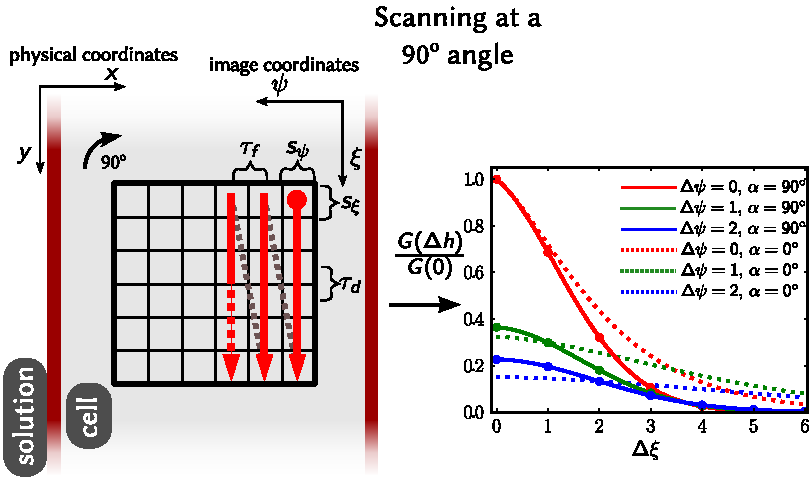
\includegraphics[width=10cm]{figures/rics_theory_3.pdf}
    \caption[Extended \acs{RICS}: scanning at an angle]{
    Modified scanning for \acs{RICS}. Scanning at an angle
    $\alpha$ rotates the image coordinates with respect to the physical
    coordinates and results in a different \ac{CF} which can be used for
    determining anisotropy of diffusion. The
    \ac{CF} for $0^\circ$ angle scanning from \F{~\ref{fig:rics_theory2}} is shown in dotted lines and differs from
    the \ac{CF} obtained for an image scanned at a different angle. In the
    shown example, scanning is performed at a $90^\circ$ angle,
    effectively aligning the image $\xi$ axis with the physical $y$ axis
    and image $\psi$ axis with physical $x$ axis. 
    }
  \label{fig:rics_theory3}
\end{figure}

In order to detect anisotropy of diffusion, several scanning angles can be used to alter the time delay
between pixels acquired from the same location 
\citep{Vendelin_08_AmJPhysiolCellPhysiol_295_pC1302}. 
When scanning is performed at an angle $\alpha$ relative to the physical
coordinate axes, the \ac{CF} equations need to be modified to account for this.
For example, if scanning is performed under a 90$^\circ$ angle, the
image $\xi$ and $\psi$ axes actually correspond to the physical $y$ and
$x$ axes, respectively (see \F{~\ref{fig:rics_theory3}}).
The \ac{CF} that takes the scanning angle into
account is:
\begin{align}
  G(\Delta \mathbf{h},\alpha) &= \frac{1}{\langle c \rangle} 
  \prod_{i=1}^n\left[
  \frac{1}{\sqrt{\pi\left(4D_it(\Delta \mathbf{h})+w_i^2)\right)}}
  \exp\left(-\frac{q(\Delta \mathbf{h},\alpha)_i^2}
  {4D_it(\Delta \mathbf{h})+w_i^2}\right)\right]\,,
  \label{eq:G_alpha}
\end{align}
%\begin{align}
%  \label{eq:G_alpha}
%  G(\Delta \mathbf{h},\alpha) = \frac{1}{\langle c \rangle} 
%  \prod_{i=1}^n\left[
%  \frac{1}{\sqrt{\pi\left(4D_it(\Delta \mathbf{h})+w_i^2)\right)}}\right.\nonumber\\
%  \left.\cdot\exp\left(-\frac{\left(\mathbf{M\left(\alpha\right)}\left(\Delta \mathbf{h}\mathbf{s}^T\right)^T\right)_i^2}{4D_it(\Delta \mathbf{h})+w_i^2}\right)\right]
%\end{align}
where the physical shift $\Delta \mathbf{p}$ is now a function of the rotation
angle $\alpha$:
\begin{equation}
  \label{eq:phys_wangle}
  \Delta \mathbf{p}(\Delta \mathbf{h},\alpha) =
  \Delta \mathbf{h}\,\mathbf{S}\left(\mathbf{M}\left(\alpha\right)\right)^T
\end{equation}
$\mathbf{M}(\alpha)$ is the rotation matrix for rotation angle
$\alpha$. For rotating around the $z$ axis, as is done in this paper, the
rotation matrix is:
\begin{equation*}
  \mathbf{M}(\alpha) = 
  \begin{pmatrix}
    \cos\alpha & -\sin\alpha & 0\\
    \sin\alpha & \,\,\,\,\,\cos\alpha & 0\\
    0&0&1
 \end{pmatrix}.
\end{equation*}
It is possible to do rotations around  another  axis or even multiple
rotations around different axes by inserting a suitable rotation matrix
in \Eq{~\ref{eq:phys_wangle}}
(assuming that the microscope employed is able to perform such scans).

The physical shift vector from \Eq{~\ref{eq:phys_wangle}} for rotation
$\alpha$ around the $z$ axis is:
\begin{align*}
  \Delta \mathbf{p}(\Delta \mathbf{h},\alpha)
%  \mathbf{M}(\alpha)\left(\Delta \mathbf{h}\mathbf{S}\right)^T \\ 
&=\,\left[\Delta x , \Delta y , \Delta z\right]\\
&=
\,\Delta \mathbf{h}\mathbf{S}\left(\mathbf{M}(\alpha)\right)^T\\
&=
\begin{pmatrix}
    \Delta \xi\cdot s_\xi\\
    \Delta \psi\cdot s_\psi\\
    \Delta \zeta \cdot s_\zeta
\end{pmatrix}^T
\begin{pmatrix}
    \,\,\,\,\,\cos\alpha & \sin\alpha & 0\\
    -\sin\alpha & \cos\alpha & 0\\
    \,\,\,\,\,0&0&1
\end{pmatrix}\\
&=\begin{pmatrix}
\Delta \xi\cdot s_\xi\cdot \cos\alpha -  \Delta \psi\cdot s_\psi\cdot \sin\alpha\\
\Delta \xi\cdot s_\xi\cdot \sin\alpha + \Delta \psi\cdot s_\psi\cdot \cos\alpha \\
\Delta \zeta\cdot s_\zeta
\end{pmatrix}^T.
\end{align*}
It is easy to verify that when $\alpha=0$,  $\mathbf{M}$ reduces to the
identity matrix and \Eq{~\ref{eq:G_alpha}} simplifies to
\Eq{~\ref{eq:G_0angle}}.


\subsection{Variation of scanning resolution}
Changes in scanning resolution
\citep{Vendelin_08_AmJPhysiolCellPhysiol_295_pC1302} or pixel dwell time
$\tau_d$ \citep{Groner_10_OptExpress_18_p21225} will alter
the time delay function \Eq{~\ref{eq:timedelay}} and result in different correlation curves.
An example for scanning with double resolution but unchanged pixel dwell
time $\tau_d$ in $\xi$ axis is shown on 
\F{~\ref{fig:rics_theory4}}. An increased resolution increases the time
taken to record a line and decreases pixel
size. Therefore, in order to compare the \ac{CF} for different
resolutions it is more suitable to present them as functions of physical
distance as is done in \F{~\ref{fig:rics_theory4}}. 

\begin{figure}
  \centering
    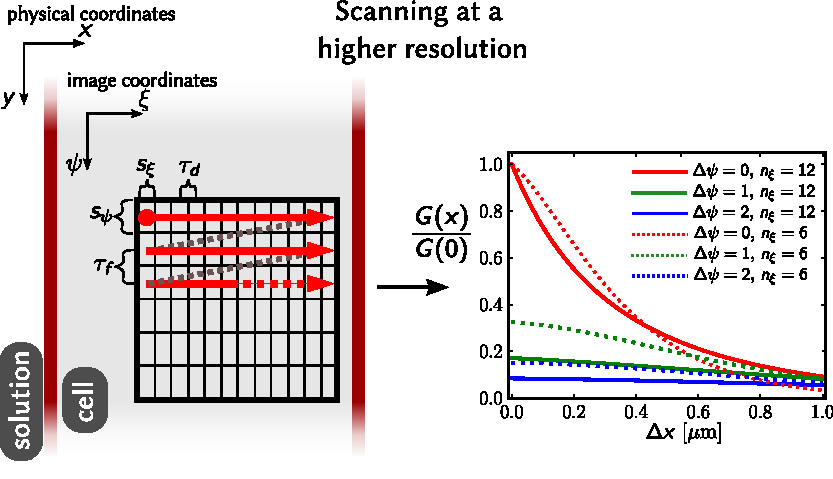
\includegraphics[width=10cm]{figures/rics_theory_5.pdf}
    \caption[Extended \acs{RICS}: changing scanning resolution]{
    Modified scanning for \acs{RICS}. Changing the
    scanning resolution also alters the shape of the \ac{CF}. In the example
    shown, the image is scanned at two times higher resolution resulting
    in the \ac{CF} depicted with solid lines. Since the pixel dwell time
    $\tau_d$ is not changed, scanning one line takes two times longer. For comparison, the \ac{CF} from
    \F{~\ref{fig:rics_theory2}} is shown in dotted lines. The horizontal
    axis now shows physical shift values in $\mu$m since the pixel size and count
    for the two \acp{CF} is different.
    }
  \label{fig:rics_theory4}
\end{figure}

\subsection{\newtext{Two diffusing species}}
It is possible for the fluorescent molecule to bind with other, larger, molecules
in the intracellular solution. As a result, two subspecies of
the fluorescent molecule would be diffusing in the cell: the faster unbound form
and the slower bound form. Assuming that fluorescent properties of the
dye are not altered as a result of binding and that the two species are
non-interacting (\ie, the binding/unbinding is relatively slow),
the \ac{CF} for two species diffusing is \citep{Lakowicz_06_Springer,Krichevsky_02_ReportsonProgPhys_65_p251} :
\begin{align}
G(\Delta \mathbf{h},\alpha)&=\frac{1}{\langle
c_1(\mathbf{p})+c_2(\mathbf{p})\rangle_{\mathbf{p}}^2}\nonumber\\
&\cdot\int\!\!\int
W(\mathbf{r})W(\mathbf{r'})
\left(
\langle c_1 \rangle \cdot g_{D1}
+
\langle c_2 \rangle \cdot g_{D2}
\right)
\dd \mathbf{r}\dd \mathbf{r'},
\label{eq:G_2c}
\end{align}
where $\langle c_1 \rangle$, $\langle c_2 \rangle$ are concentrations of
the two components and $g_{D1}$ and $g_{D2}$ are given by
$G_{Dk}(\mathbf{r},\mathbf{r'},\Delta \mathbf{h},\alpha) / \langle c_k
\rangle$, ($k=$1, 2).
Inserting the gaussian \ac{PSF} given in \Eq{~\ref{eq:PSF_def}} to calculate the \ac{CF} for two
components from \Eq{~\ref{eq:G_2c}}:
\begin{align*}
  G(\Delta \mathbf{h},\alpha) &= \frac{1}{\left(\langle c_1 \rangle+
  \langle c_2 \rangle\right)^2}\\
  &\cdot\bigg[\langle c_1 \rangle\prod_{i=1}^n
  \frac{
  \exp\left(-\frac{q(\Delta \mathbf{h},\alpha)_i^2}
  {4D_{1,i}t(\Delta \mathbf{h})+w_i^2}\right)
  }{\sqrt{\pi\left(4D_{1,i}t(\Delta \mathbf{h})+w_i^2)\right)}}\\
  &+\langle c_2 \rangle\prod_{i=1}^n
  \frac{
  \exp\left(-\frac{q(\Delta \mathbf{h},\alpha)_i^2}
  {4D_{2,i}t(\Delta \mathbf{h})+w_i^2}\right)
  }{\sqrt{\pi\left(4D_{2,i}t(\Delta \mathbf{h})+w_i^2)\right)}}\bigg]
  \,,
  \label{eq:G_alpha}
\end{align*}
where $D_{1,i}$, $D_{2,i}$  are diffusion coefficients in direction $i$ for the first and second component,
respectively. 

\subsection{\newtext{Triplet states}}
It is possible for a fluorescent molecule to go into a so-called triplet
state from where it relaxes back to ground state after a delay much
longer than it takes for the normal excitation-emission cycle to
complete. This phenomenon, if ignored, could cause diffusion coefficients to be
overestimated. To account for this effect, we multiply the \ac{CF} function
(\Eq{~\ref{eq:G_alpha}} or \Eq{~\ref{eq:G_2c}} )
with a compensation factor
\citep{Widengren_95_JPhysChem_99_p13368,Krichevsky_02_ReportsonProgPhys_65_p251,Haustein_07_AnnuRevBiophysBiomolStruct_36_p151,Groner_10_OptExpress_18_p21225} :
\begin{equation}
  1+\frac{T}{1-T}\exp\left(-\frac{t}{\tau}\right),
\end{equation}
where $T$ is the fraction of molecules in triplet state and $\tau$ the
triplet state relaxation time. 


\section{\newtext{Full form of correlation function}}
In this work the experimentally measured 
\ac{PSF} was used instead of the approximated one (\Eq{~\ref{eq:PSF_def}}), necessitating numerical integration for
each \ac{CF} evaluation:
\begin{align}
G(\Delta \mathbf{h},\alpha)&=\frac{1}{\langle
F_1(\mathbf{p})+F_2(\mathbf{p})\rangle_{\mathbf{p}}^2}
\left(
1+\frac{T}{1-T}\exp\left(-\frac{t}{\tau}\right)
\right)
\nonumber\\
&\cdot\int\!\!\int
W(\mathbf{r})W(\mathbf{r'})
\left(
\langle c_1 \rangle \cdot g_{D1}
+
\langle c_2 \rangle \cdot g_{D2}
\right)
\dd \mathbf{r}\dd \mathbf{r'}
\label {eq:G_2ctrip}
\end{align}

This is the \ac{CF} form used for fitting experimental data in this work.
